\documentclass{beamer}
\usepackage[utf8]{inputenc}
\usepackage{graphicx}
\usepackage{tikz}
\usepackage{xcolor}
% TIKZ TEMPLATE STARTED
\usetikzlibrary{shapes.geometric, arrows}
\tikzstyle{startstop} = [rectangle, rounded corners, minimum width=3cm, minimum height=1cm, text centered, draw=black, fill=red!30]
\tikzstyle{gnode} = [circle, minimum width=.35cm, minimum height=.35cm, text centered, draw=black, fill=red!30]
\tikzstyle{gleaf} = [circle, minimum width=1cm, minimum height=1cm, text centered, draw=black, fill=green!30]
\tikzstyle{gleaf2} = [circle, minimum width=1cm, minimum height=1cm, text centered, draw=black, fill=blue!30]
\tikzstyle{io} = [trapezium, trapezium left angle=70, trapezium right angle=110, minimum width=3cm, minimum height=1cm, text centered, draw=black, fill=blue!30]
\tikzstyle{process} = [rectangle, minimum width=3cm, minimum height=1cm, text centered, text width=3cm, draw=black, fill=orange!30]
\tikzstyle{textonly} = [rectangle, minimum width=1cm, minimum height=1cm, text center, text width=1cm, draw=white, fill=white]
\tikzstyle{decision} = [diamond, minimum width=3cm, minimum height=1cm, text centered, draw=black, fill=green!30]
\tikzstyle{arrow} = [thick,->,>=stealth]
\tikzstyle{place}=[circle,draw=blue!50,fill=blue!20,thick]
\tikzstyle{visited} = [circle, draw, red!50, fill=green!20,thick]
\tikzstyle{current} = [circle, draw, red!50, fill=blue!20,thick]
% TIKS TEMPLATE ENDED
% \usetheme{Madrid}

\title{Class 2 - TiKZ}
\subtitle{MeoMOe}
\author[N. N]{No Name}
\institute[CSE, BUET]{
    Department of Computer Science and Engineering\\
    Bangladesh University of Engineering and Technology
}
% \logo{\includegraphics[height=1cm]{}}
\date{\today}

\begin{document}
\begin{frame}{}
\maketitle
\end{frame}

\begin{frame}{Tikz}
    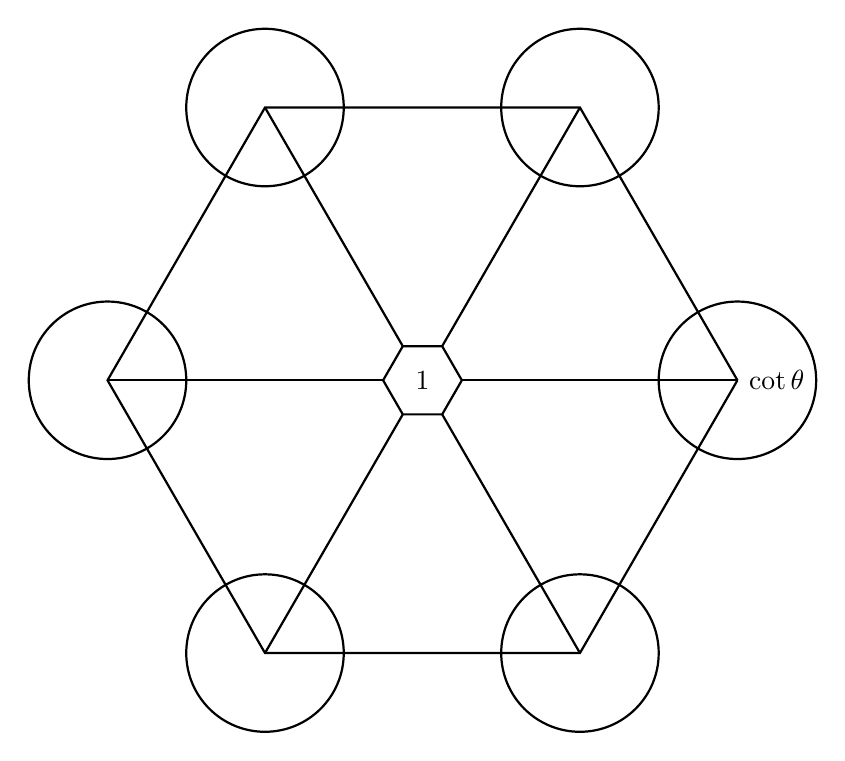
\begin{tikzpicture}
    \draw[thick] (0:4) -- (60:4) -- (120:4) -- (180:4) -- (240:4) -- (300:4) -- (360:4);
    \draw[thick] (0:.5) -- (60:.5) -- (120:.5) -- (180:.5) -- (240:.5) -- (300:.5) -- (360:.5);
    
    % \draw[thick] (0:4) -- (0:.5);
    % \draw[thick] (60:4) -- (60:.5);
    % \draw[thick] (120:4) -- (120:.5);
    % \draw[thick] (180:4) -- (180:.5);
    % \draw[thick] (240:4) -- (240:.5);
    % \draw[thick] (300:4) -- (300:.5);
    % loooooooooop
    \foreach \x in {0,60,120,180,240,300}{
        \draw[thick] (\x:4) -- (\x:.5);
        \draw[thick] (\x:4) circle(1);
    }
    
    \node at (0, 0) (1){1};
    \node at (0:4.5) (cot){$\cot\theta$};
    
    
     
    
    
    
    \end{tikzpicture}
\end{frame}


\end{document}